\documentclass{article}

\usepackage{graphicx, xcolor}
\usepackage{amsmath, amssymb}
\usepackage{float}
\usepackage[colorlinks=true,allcolors=blue]{hyperref}

\usepackage[margin=1in]{geometry}

\def\hwtitle{Homework 7: The Bootstrap Method}
\def\hwauthor{Caden Gobat}
\def\hwdate{\today}

\usepackage{fancyhdr}
\lhead{\hwauthor}
\chead{\hwtitle}
\rhead{\hwdate}
\lfoot{\hwauthor}
\cfoot{}
\rfoot{\thepage}
\renewcommand{\footrulewidth}{0.4pt}
\pagestyle{fancy}

\author{\hwauthor}
\title{\hwtitle}
\date{\hwdate}

\begin{document}

\maketitle
\thispagestyle{fancy}

\section{Introduction}

In this assignment, address the ubiquitous problem of fitting an analytical function to discrete/numerical data. To do this, we will attempt to minimize a $\chi^2$ (chi-squared) goodness-of-fit measure to optimize a set of coefficients on a polynomial. The $\chi^2$ statistic is defined as \begin{equation*}
    \chi^2 \equiv \sum_i \frac{(P(x_i)-y_i)^2}{\sigma_i^2}
\end{equation*}
Where $P(x)$ is a fitted polynomial function and $x$, $y$, and $\sigma$ are the independent quantity, dependent quantity, and standard error in $y$, respectively. We will use this value to determine whether certain models appropriately describe our data.

\section{Results}

\bigskip
\noindent{\bf Question 1}
\medskip

\begin{figure}[H]
    \centering
    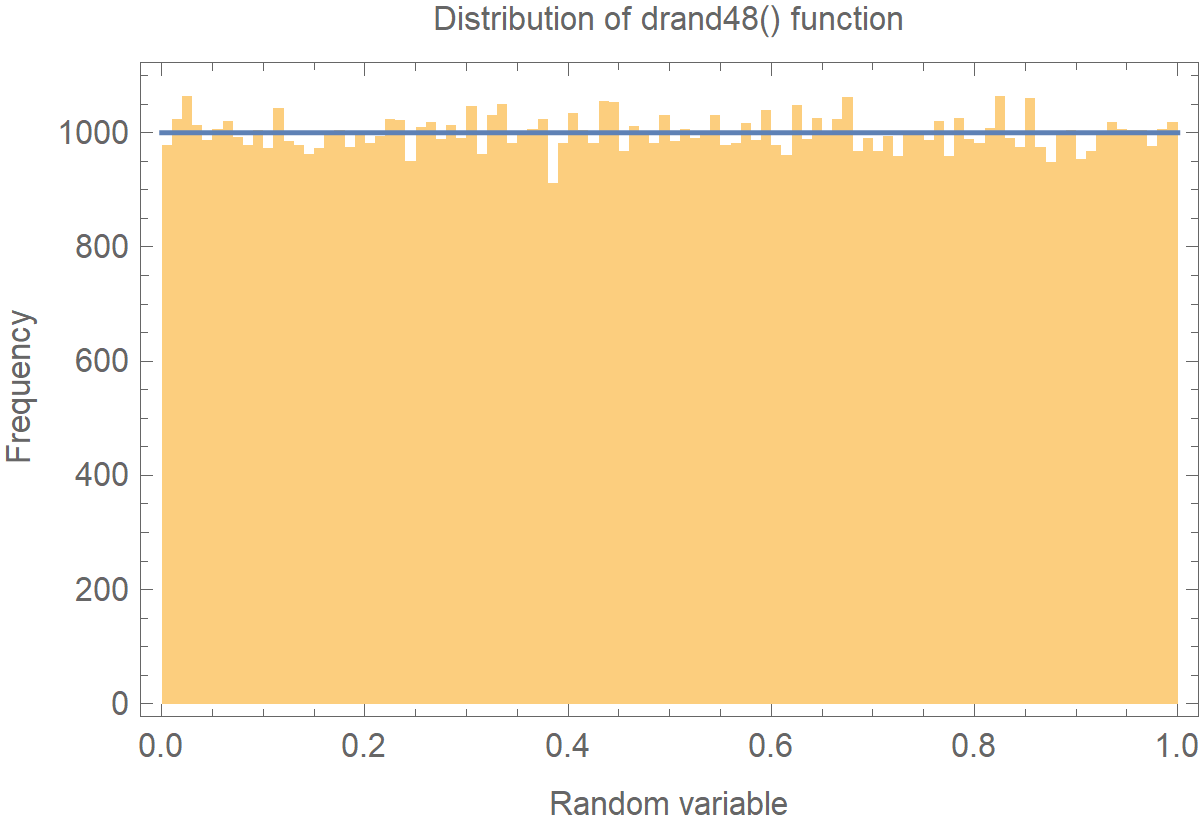
\includegraphics[width=4.4in]{homework7/uniform_dist.png}
    \caption{100-bin histogram (in gold) with 100 bins of 100,000 random numbers generated using \texttt{C}'s \texttt{drand48()} function. As expected, this conforms relatively closely to a uniform distribution of floating point numbers between 0 and 1, the PDF of which is shown in blue.}
    \label{fig:drand48}
\end{figure}

\begin{figure}[H]
    \centering
    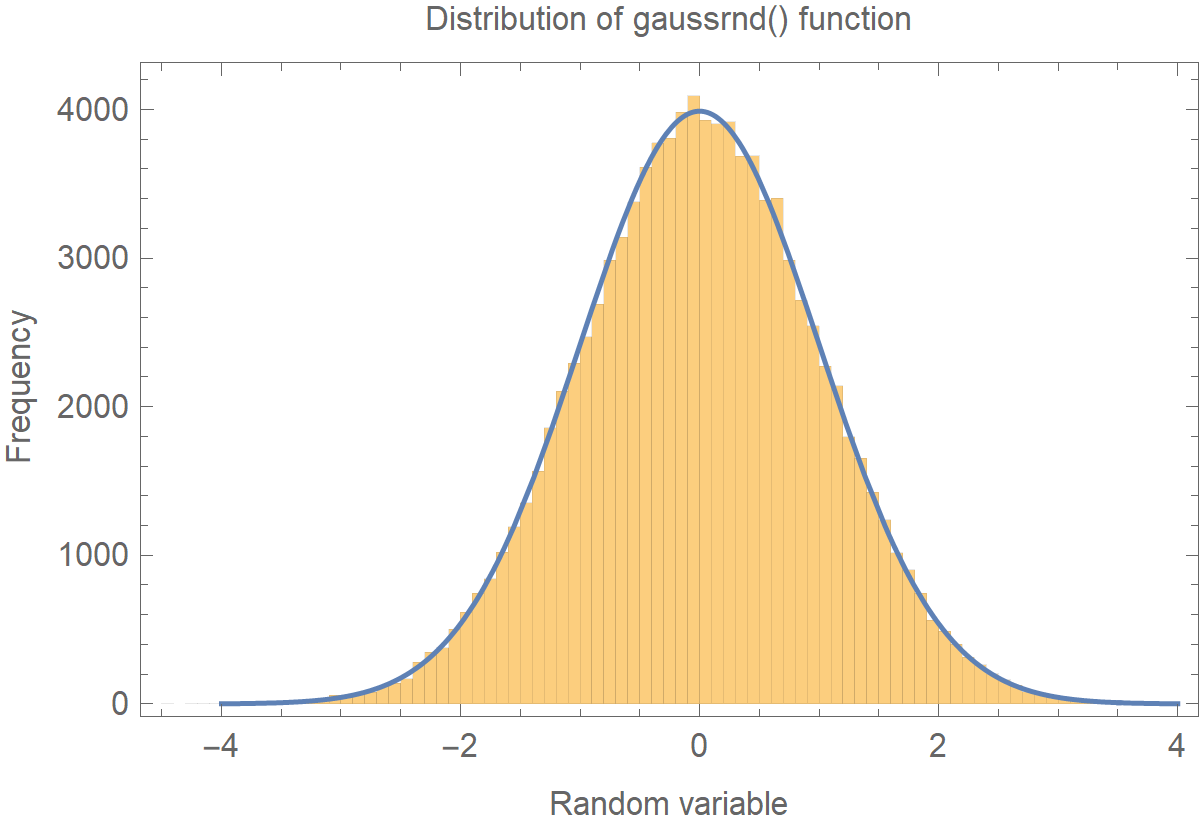
\includegraphics[width=4.4in]{homework7/normal_dist.png}
    \caption{100-bin histogram (in gold) of 100,000 random numbers generated using our \texttt{gaussrnd()} function. As expected, this conforms quite closely to a normal distribution with $\mu=1$ and $\sigma=1$, the PDF of which is shown in blue.}
    \label{fig:gaussrnd}
\end{figure}

\bigskip
\noindent{\bf Question 2}
\medskip

\begin{figure}[H]
    \centering
    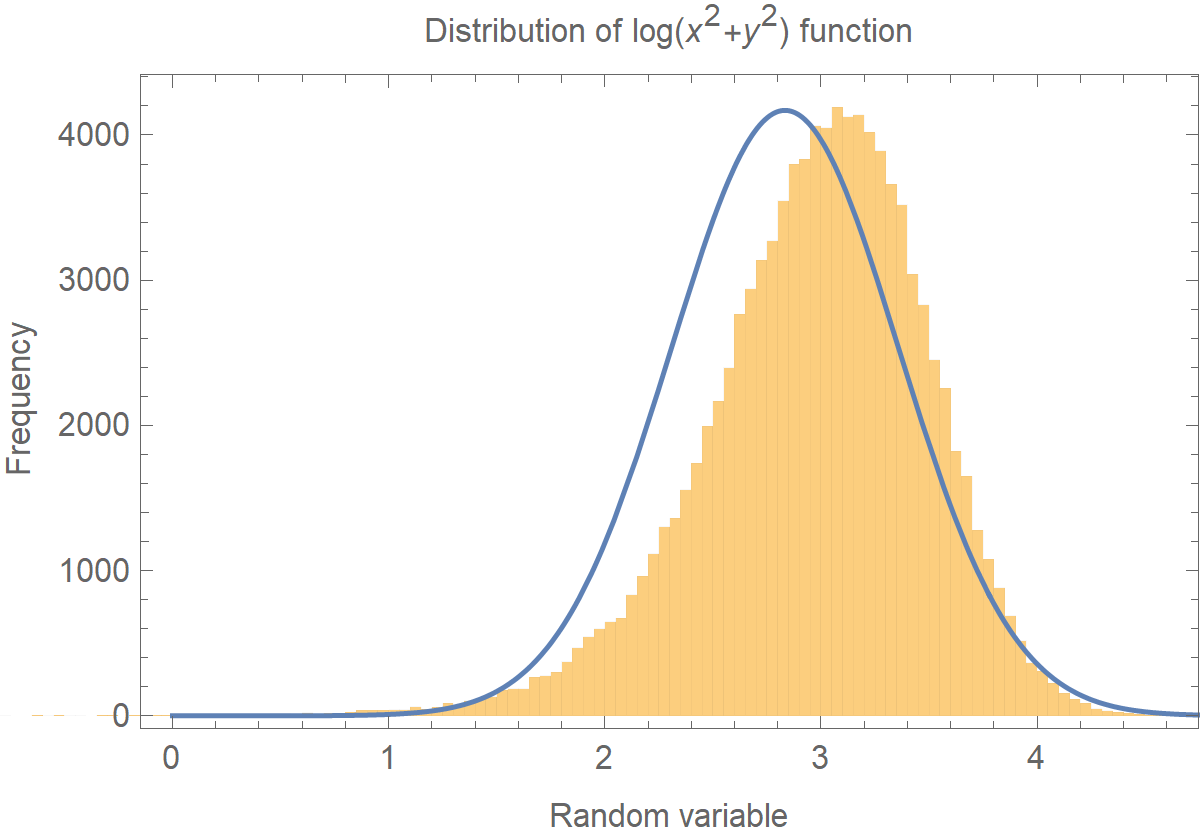
\includegraphics[width=4.4in]{homework7/log_dist.png}
    \caption{100-bin histogram (in gold) of 100,000 randomly generated numbers from the distribution $\log(x^2+y^2)$, where $x$ and $y$ are each uniformly-distributed variables with $\bar{x}=1$, $\bar{y}=4$, $\sigma_x=2$, and $\sigma_y=1$. The PDF of a normal distribution with $\mu=\log(1^2+4^2)=\log(17)$ and $\displaystyle \sigma^2=\left(\left.\frac{\partial f}{\partial x}\right|_{\bar{x},\bar{y}}\right)^2\sigma_x^2 + \left(\left.\frac{\partial f}{\partial y}\right|_{\bar{x},\bar{y}}\right)^2\sigma_y^2 = \frac{16\bar{x}^2}{(\bar{x}^2+\bar{y}^2)^2}+\frac{4\bar{y}^2}{(\bar{x}^2+\bar{y}^2)^2}=\frac{80}{289}$. This PDF is in less agreement with the distribution than in the previous problem because the logarithm throws off the normality of the selection. Although $x$ and $y$ are each normally distributed, taking the logarithm of their squared sum creates a sample of numbers that are not normal, so trying to ascribe a Gaussian function with $\mu$ and $\sigma$ using this analytical technique is invalid.}
    \label{fig:logx2y2}
\end{figure}

\bigskip
\noindent{\bf Question 3}
\medskip

An alternative formula for calculating a $\chi^2$ statistic is \begin{equation*}
    \chi^2 = \sum_{i=1}^N \frac{(\bar{x_i}-x_i)^2}{\bar{x_i}}
\end{equation*}
which does not rely on the data coming with any error $\sigma$. However, being able to calculate a chi-squared value for these data does not mean that we will necessarily get a good fit. Radioactive decay behaves exponentially, not as a polynomial, so we have more fundamental issues with our methodology. Second- and third- order polynomials do not even come close visually to fitting the data. A fourth-order polynomial with coefficients \begin{equation*}
    0.0193t^4 - 3.931t^3 + 295.364t^2 - 9923.637t + 131394.55
\end{equation*}
comes within the realm of feasibility, providing the fit shown in Fig.~\ref{fig:decay}. This yields $\chi^2=1606.5$ and we have 20 data points in \texttt{decay.dat}, so there are $20-5=15$ degrees of freedom in this fit. Therefore the reduced $\chi^2$ is $\chi_\nu^2 \cong 107.1$. This is still very poor. There is a chance that moving up to higher order polynomials may improve this, but a much better option would be to change the underlying model itself. For example, using an exponential model with fitted parameters \begin{equation*}
    133565e^{-0.086t}
\end{equation*}
gives $\chi^2=12.2$ with $\chi_\nu^2 = 0.677$. This is an improvement of two orders of magnitude, and requires fewer parameters to attain a much better fit. Therefore we can conclude that this is a better fundamental model. 

We can determine the half life by solving $\displaystyle 0.5 = e^{-0.086t}$. This yields $\ln(0.5)=-0.086t \implies t = 8.06$ days, or around 696000 seconds. This matches most closely with iodine-131, which has a half life of approximately 693 ks.

\begin{figure}[H]
    \centering
    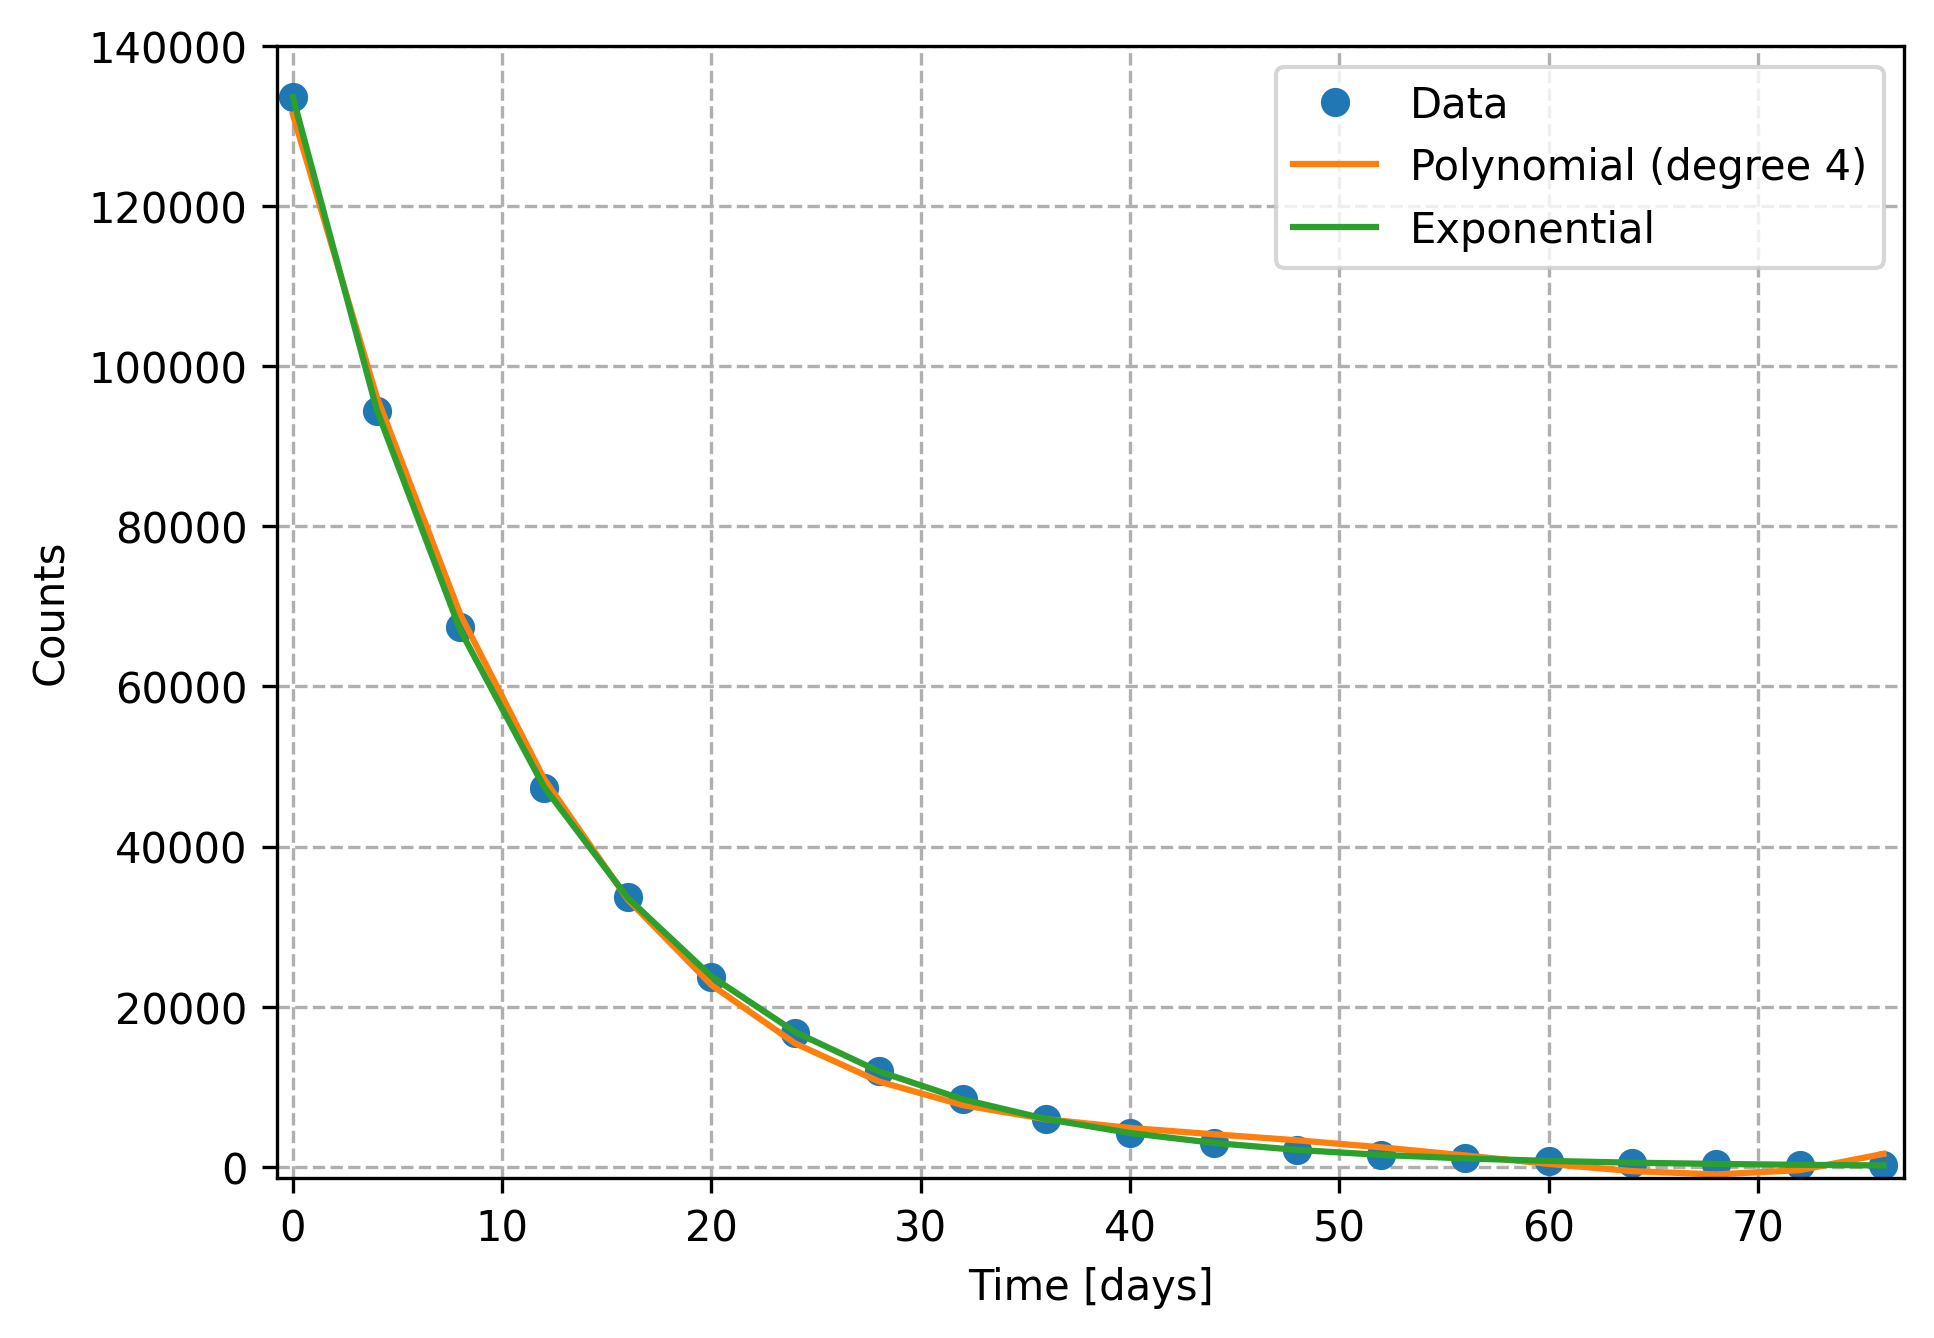
\includegraphics[width=6in]{homework6/decay.png}
    \caption{Radioactive decay data with two models fitted. Parameters for each model are those given above, with the exponential fit being decidedly better.}
    \label{fig:decay}
\end{figure}

\section{Conclusions}

I greatly enjoyed this assignment, and I have a much better understanding of the mechanism behind $\chi^2$ analysis now, having built a fitting engine from the ground up. I also appreciated learning the underlying statistical theory of confidence levels and distributions.

I am curious about how one might deal with errors in the horizontal direction (i.e. an error on the $x$-values as well), and am looking forward to continuing to work on these kinds of problems.

\end{document}
